%\subsubsection{Standard deviation vs blocking error}
%An example result of the mean energy using the standard deviation of the error in the non-interacting case with 10 3-dimensional particles with $\alpha = 0.4$ is $E = 15.3691 \pm 0.0009$. This error is unrealistically small. By applying blocking, we get an error of $\pm 0.02$. It is obvious that the blocking error gives a better estimate since it takes into account the time-series correlation of the dataset. Therefore all errors presented in this project will be calculated by applying the blocking method to our data sets. 

\subsection{No boson-boson interaction}
We gather data using two methods: brute force Metropolis and Importance Sampling algorithms. 

\subsubsection{Brute force Metropolis}
%As discussed in \ref{analysis of hamiltonian}, in both interacting and non cases, we have an analytical expression for the local energy. Nevertheless at the beginning of the developing of the program, it is useful to benchmark the computation with a different approach. With such a spirit we used a numerical derivative to compute the kinetic energy. This approach is much slower than the analytical evaluation: the time required to perform numerical derivative is at least twice than the one spent for the analytical one as it is possible to see from Tab. \ref{tab_brute_times_1}. 
In this first part of the project, we use the brute force Metropolis algorithm as method to choose new moves (eq. (\ref{eq_accept_move})). From Tab. \ref{tab_brute_energy} we can state that our code is successful in computing the local energy. The accuracy of the analytical energy is perfect as we would aspect.. The length step used in all this computations is determined in a really roughly way by trial and errors. In our case we find $L=1.0$ to be an appropriate value for our aims. 

From Tab. \ref{tab_brute_energy} we note also the drawback of this brute force Metropolis which is the relative low acceptance rate (about $\sim 74\ \si{\percent}$): this means that we lose an important amount of time by proposing moves which get rejected. To avoid this issue, the Importance Sampling is implemented.


\begin{table}[H]
\caption{Energy of the many-particle boson system in three dimensions obtained using Brute-Force Metropolis algorithm compared with the exact results calculated from eq. (\ref{eq_energy_noninter_result}). Note the relative low acceptance ratio.}
\centering
\begin{tabular}{l l |c c c} 
\textbf{N} & \textbf{d}  & \textbf{Exact energy} & \textbf{Analytical energy} & \textbf{Acceptance ratio} \\\hline 
1 & 3& 1.5 &  $1.5\pm0.0$ & 0.74 \\ 
10 & 3& 15 & $15\pm0$ & $0.74$\\
100 & 3&150 & $150\pm0$ & $0.74$ \\
500 & 3&750 & $750\pm0$  & $0.74$\\ 
\end{tabular}
\label{tab_brute_energy}
\end{table} 



%For example 100 particle 3 dim with analytic solution and alpha = 4. Mean is 153.584 and stdev is 2.779. With blocking st dev is 0.1659.


\subsubsection{Importance Sampling}
We implement the Importance Sampling with the acceptance rule shown previously in eq. (\ref{eq_imp_sam}). To check whether our implementation is correct we compare the local energy obtained with different variational parameter $\alpha$ with the Brute Force Metropolis and the Importance Sampling method. From Tab. \ref{tab_imp_samp} we don't note relevant differences between the two sets of data except the error which is usually more in the importance sampling case. Furthermore 
the minimum of the local energy with respect to $\alpha$ is clearly in $0.5$ where all the methods flow into perfectly. This shown once again the goodness of the procedures adopted.
%These sets of data are also plotted in Fig. (\ref{fig_energy_minimum}) where the length of the vertical lines represents the uncertainty on the data. As we expect from the theory, the minimum of the local energy with respect to $\alpha$ is clearly in $0.5$ where all the methods flow into perfectly. This shown once again the goodness of the procedures adopted.

\begin{table}[H] \centering
	\caption{Local energy for the $10$ particle case in three dimensions with Brute force Metropolis and Importance Sampling. The results are produced using $10^6$ MC cycles.}
	\begin{tabular}{l |c |c } 
		$\alpha $&\hfill \textbf{Brute Force Metropolis} \hfill & \textbf{Importance Sampling} \\ \hline
		0.40 & $15.37\pm 0.02$   & $15.40\pm 0.04$ \\
		0.45 &  $15.09\pm0.01$   & $15.06\pm0.02$  \\
		0.50 & $15.00 \pm 0.0$   &$15.00\pm 0.0$    \\
		0.55 & $15.06 \pm0.01 $  & $15.06 \pm0.01 $  \\
		0.60 & $15.26\pm0.01 $   & $15.27\pm0.02$    
		\\ 
	\end{tabular}
	\label{tab_imp_samp}
\end{table} 
All the data mentioned above are obtained by using a $\Delta t=0.01$. We decide to perform a further analysis on the value of $\Delta t$ since the use of the value $0.01$ was completely due to trial and errors experiments. Therefore we compute the local energy for $\alpha =0.4$ with several values of $\Delta t$ from $1$ to $10^{-5}$. We find the best interval with three consideration: the smoothness of the local energy during time (MC cycles), the acceptance rate of the moves and the uncertainty. The first one can be evalueted from Fig. (\ref{fig_imp_samp}), where we note how the function local energy becomes flatter as the time step decrease or in another way the noise is less. Here good choices of time steps seem $0.1,0.01,0.001,0.0001$. The last one is excluded because the method moves the particle so close that the configuration doesn't really change from the initial one i.e. it is totally biased by how the random decides to put the particles at the beginning and thus it is not to be trusted. The acceptance ratio can be evaluated in Tab. (\ref{tab_imp_acc}). Brute force MC sampling accepted around 73-74\% of the moves proposed by the algorithm, by adding the importance sampling the acceptance rate is boosted to $97-98\%$. On the other hand, at the lowest step, the system accepts all the moves since the particles are moved too close to the previous positions as explained above. Whereas the opposite happens to the largest steps. From the table but better from Fig. (\ref{fig_energy_timestep}), we can note how the uncertainties tend to increase as $\Delta t$ is lowered, a consequence of the increasing correlation of data, with the exception of the lowest value which, however, we tend to exclude from the motives already explained. From these considerations, $\Delta t\in [0.01, 0.1]$. From our purposes, we stick with the choice made before of $\Delta t =0.01$.





%\begin{figure}[H]
%\centering
%\centerline {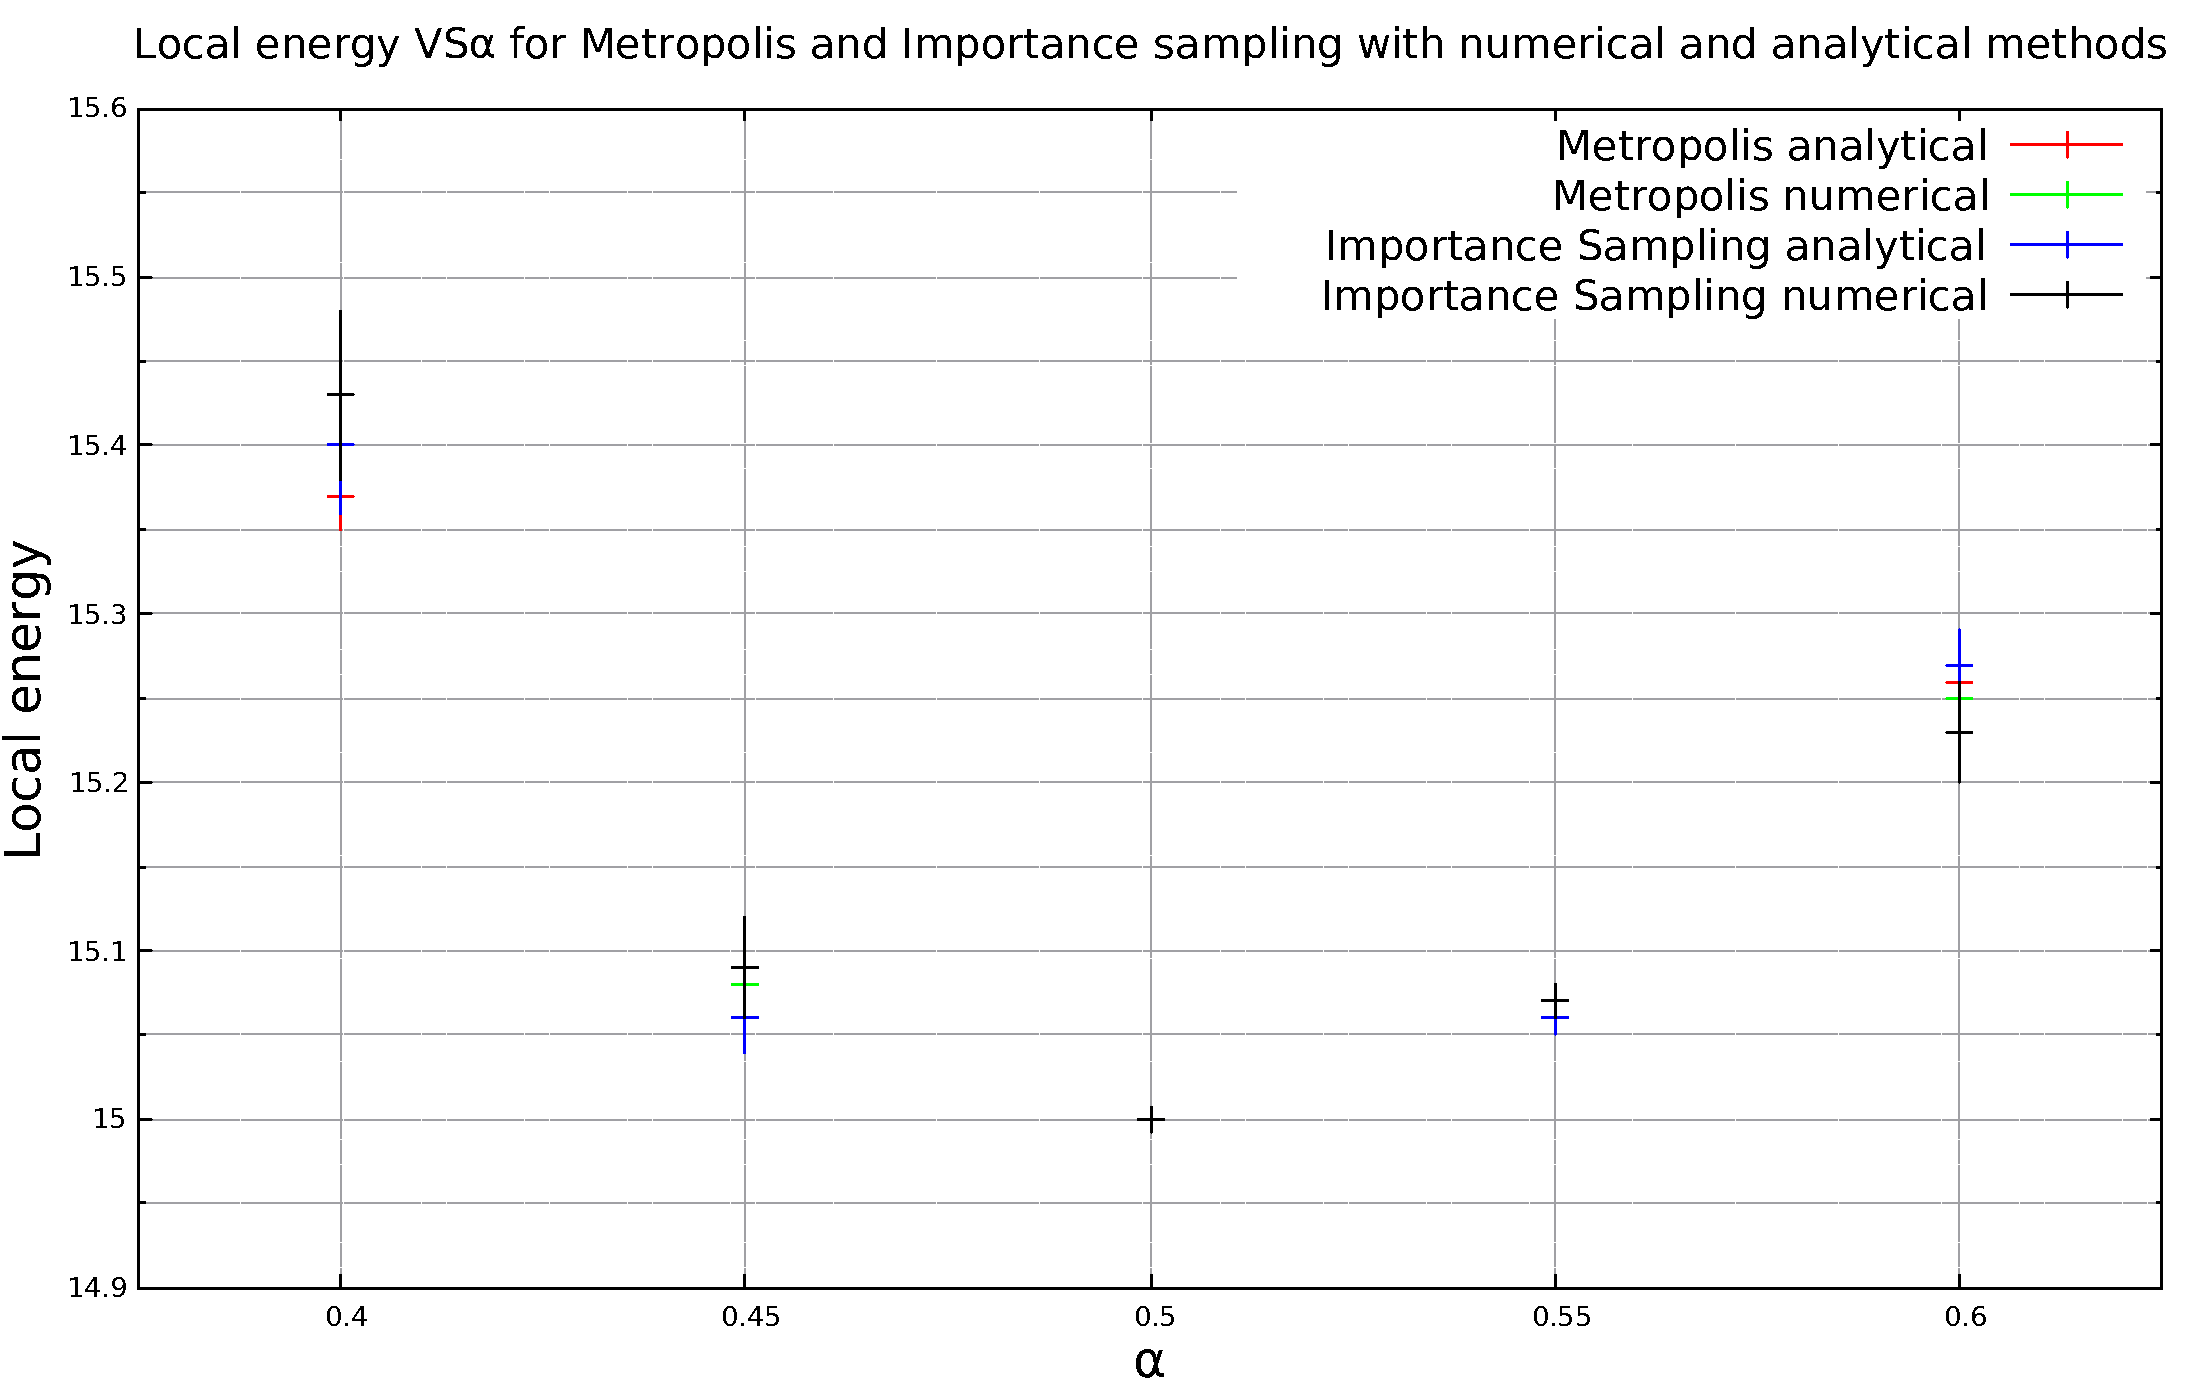
\includegraphics[scale=0.38]{figures/metro_imp}}
%\caption{Plot of the local energies from Tab. \ref{tab_imp_samp} as function of $\alpha$ for Metropolis and Importance Sampling ($\Delta t=0.01$) with numerical and analytical evaluation of energy. $10$ particles in $3D$ are used.}
%\label{fig_energy_minimum}
%\end{figure}



%Fig. \ref{fig_imp_samp} shows the instantaneous energy when applying the importance sampling methods. The curve is much smoother than the results were from the brute force MC methods. Fig. \ref{fig_imp_samp} also shows the dependency on the importance sampling timestep $\Delta t$. The energy fluctuations increase with increasing $\Delta t$. That is not to say that a smaller $\Delta t$ will always give a better result. With small $\Delta t$, the energy can randomly dip to lower values and because of its slower response, it will have trouble returning to it's actual value. 

\begin{figure}[H]
\centering
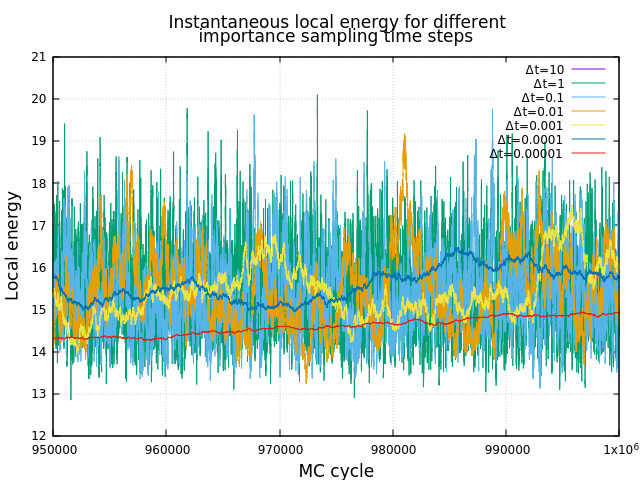
\includegraphics[scale = 0.75]{figures/importance_sampling_dt}
\caption{Variations in instantaneous local energy for various importance sampling $\Delta t$ with $\alpha = 0.4$. The energy curve fluctuations are really big for $\Delta t \geq 0.1$}
\label{fig_imp_samp}
\end{figure}





\begin{table}[H]
\caption{In the table the values of local energy and acceptance rate are reported as functions of different $\Delta t$. 10 particle case in three dimensions are considered with $10^6$ MC cycles and $\alpha =0.4$.}
\centering
\begin{tabular}{l |c |c  } 
\textbf{$\Delta t$}& \textbf{Mean local energy} & \textbf{Acceptance ratio} \\ \hline
10 & $15.14\pm 0.04$   & 0.00014   \\
1 &  $15.36\pm0.006$   & 0.68  \\
0.1 & $15.37\pm0.01$    &  0.986 \\
0.01 & $15.40 \pm0.04 $  &  0.990 \\
0.001 & $15.44\pm0.08$    &  0.994 \\
0.0001 & $15.3\pm0.1$    &  0.9997 \\
0.00001 & $14.38\pm0.04$    &  1 \\
 
\end{tabular}
\label{tab_imp_acc}
\end{table} 


\begin{figure}[H]
\centering
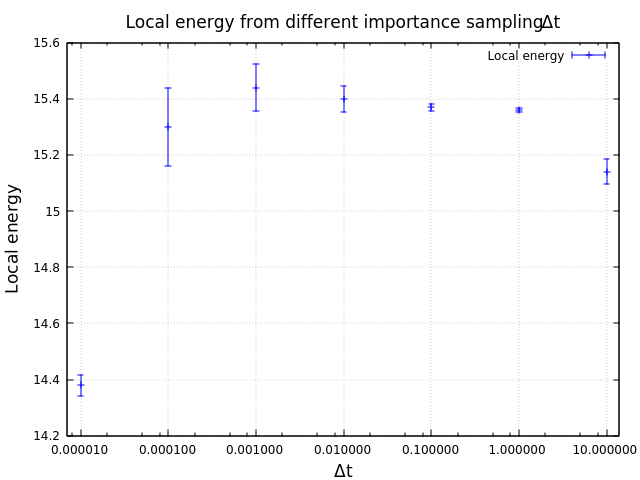
\includegraphics[scale=1]{figures/importance_sampling_dt_new}
\caption{Mean local energy computed from sets of $10^6$ MC cycles using various importance sampling $\Delta t$ with $\alpha = 0.4$ for $10$ particles in $3D$. }
\label{fig_energy_timestep}
\end{figure}

\subsection{Interacting bosons}
In this section we turn on the interaction between bosons and we trap them in an elliptic harmonic potential. The energy of the systems of interacting particles in $3$ dimensions is computed and presented in table \ref{tab_energies_inter} together with benchmark energies retrieved from Pederiva and Isacchini's article \cite{giovanni}. %They claim to have extracted the benchmarks from \cite{vmcarticle}, but how they were retrieved is not understood.

As we can see, our results follow the behaviour shown by the benchmark even though for the majority of cases our results are not compatible with them (Fig. (\ref{fig_benchmark})). We note that for $10$ particles we overestimate the results whereas for the other sets of particles we underestimate them. We do not know why it happens, but we can state that if we would have a variational parameter also in the expression of the Jastrow factor, we would probably be able to find better results. 
Nevertheless, by looking at the plot in Fig. (\ref{fig_en_alfa}) we can already safely say that the optimal parameter $\alpha$ would be in an interval around $\alpha=0.5$ which will be better inspected with the Gradient Descent method in next section.

%Figure \ref{fig_benchmark} shows the benchmark energies together with the computed energies for 100 interacting particles. The figure shows that the energies follow the tendency of the benchmark, but fail to accurately predict the local energies. In most cases the blocking error is too small to.

\begin{table}[H]
\caption{Energies of interacting particles. Benchmark results taken from \cite{giovanni}.}
\centering
\begin{tabular}{ c c c c c c  c}
\textbf{N}& \hfill \textbf{10} & &\hfill \textbf{50}& & \hfill \textbf{100} \\ \hline
\textbf{$\alpha$}  & \textbf{Benchmark} & \textbf{Result} & \textbf{Benchmark} & \textbf{Result}  &\textbf{Benchmark} & \textbf{Result}\\\hline 
$0.2$ & $34.9$ &  $35.3\pm 0.3$ & $175$ & $174\pm 1$ &  $353$   & $343.2\pm 2.1$\\ 
0.3 & 24.7 & $27.7\pm 0.1$ & 138 & $136.4\pm 0.6$ &  278   & $279.0\pm 3.3$\\
0.4 & 24.2 & $24.84\pm 0.04 $ & 125 & $123.3\pm 0.3$ &  253   & $248.4\pm 0.7$\\
0.5 & 24.2 &$24.1915\pm 2\times 10^{-4}$ & 122 & $119.81\pm 0.04$ &  247   &$241.30\pm 0.02 $\\
0.6 & 24.6 &$24.55\pm 0.04$ & 125 & $121.2\pm 0.1$ &  252   &$246.4\pm 0.7$\\
0.7 & 24.5 & $25.6\pm 0.1$& 129 & $127.1\pm 0.3$ &  263  &$253.7\pm 0.9$\\
0.8 & -- & $26.8\pm 0.1$& --  & $134.5\pm 0.3$& -- & $271\pm 2$ \\ 
\end{tabular}
\label{tab_energies_inter}
\end{table} 

\begin{figure}[H]
\centering
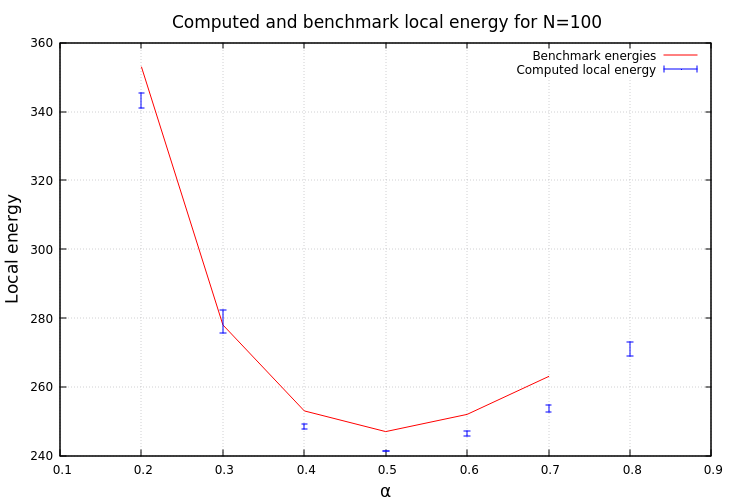
\includegraphics[scale = 0.8]{figures/compare_with_benchmark_100}
\caption{Plot of the N=100 data from Tab. \ref{tab_energies_inter}. The figure shows that the computed energies follow the tendency of the benchmarks, but they underestimate them.}
\label{fig_benchmark}
\end{figure}

\begin{figure}[H]
\centering
\centerline{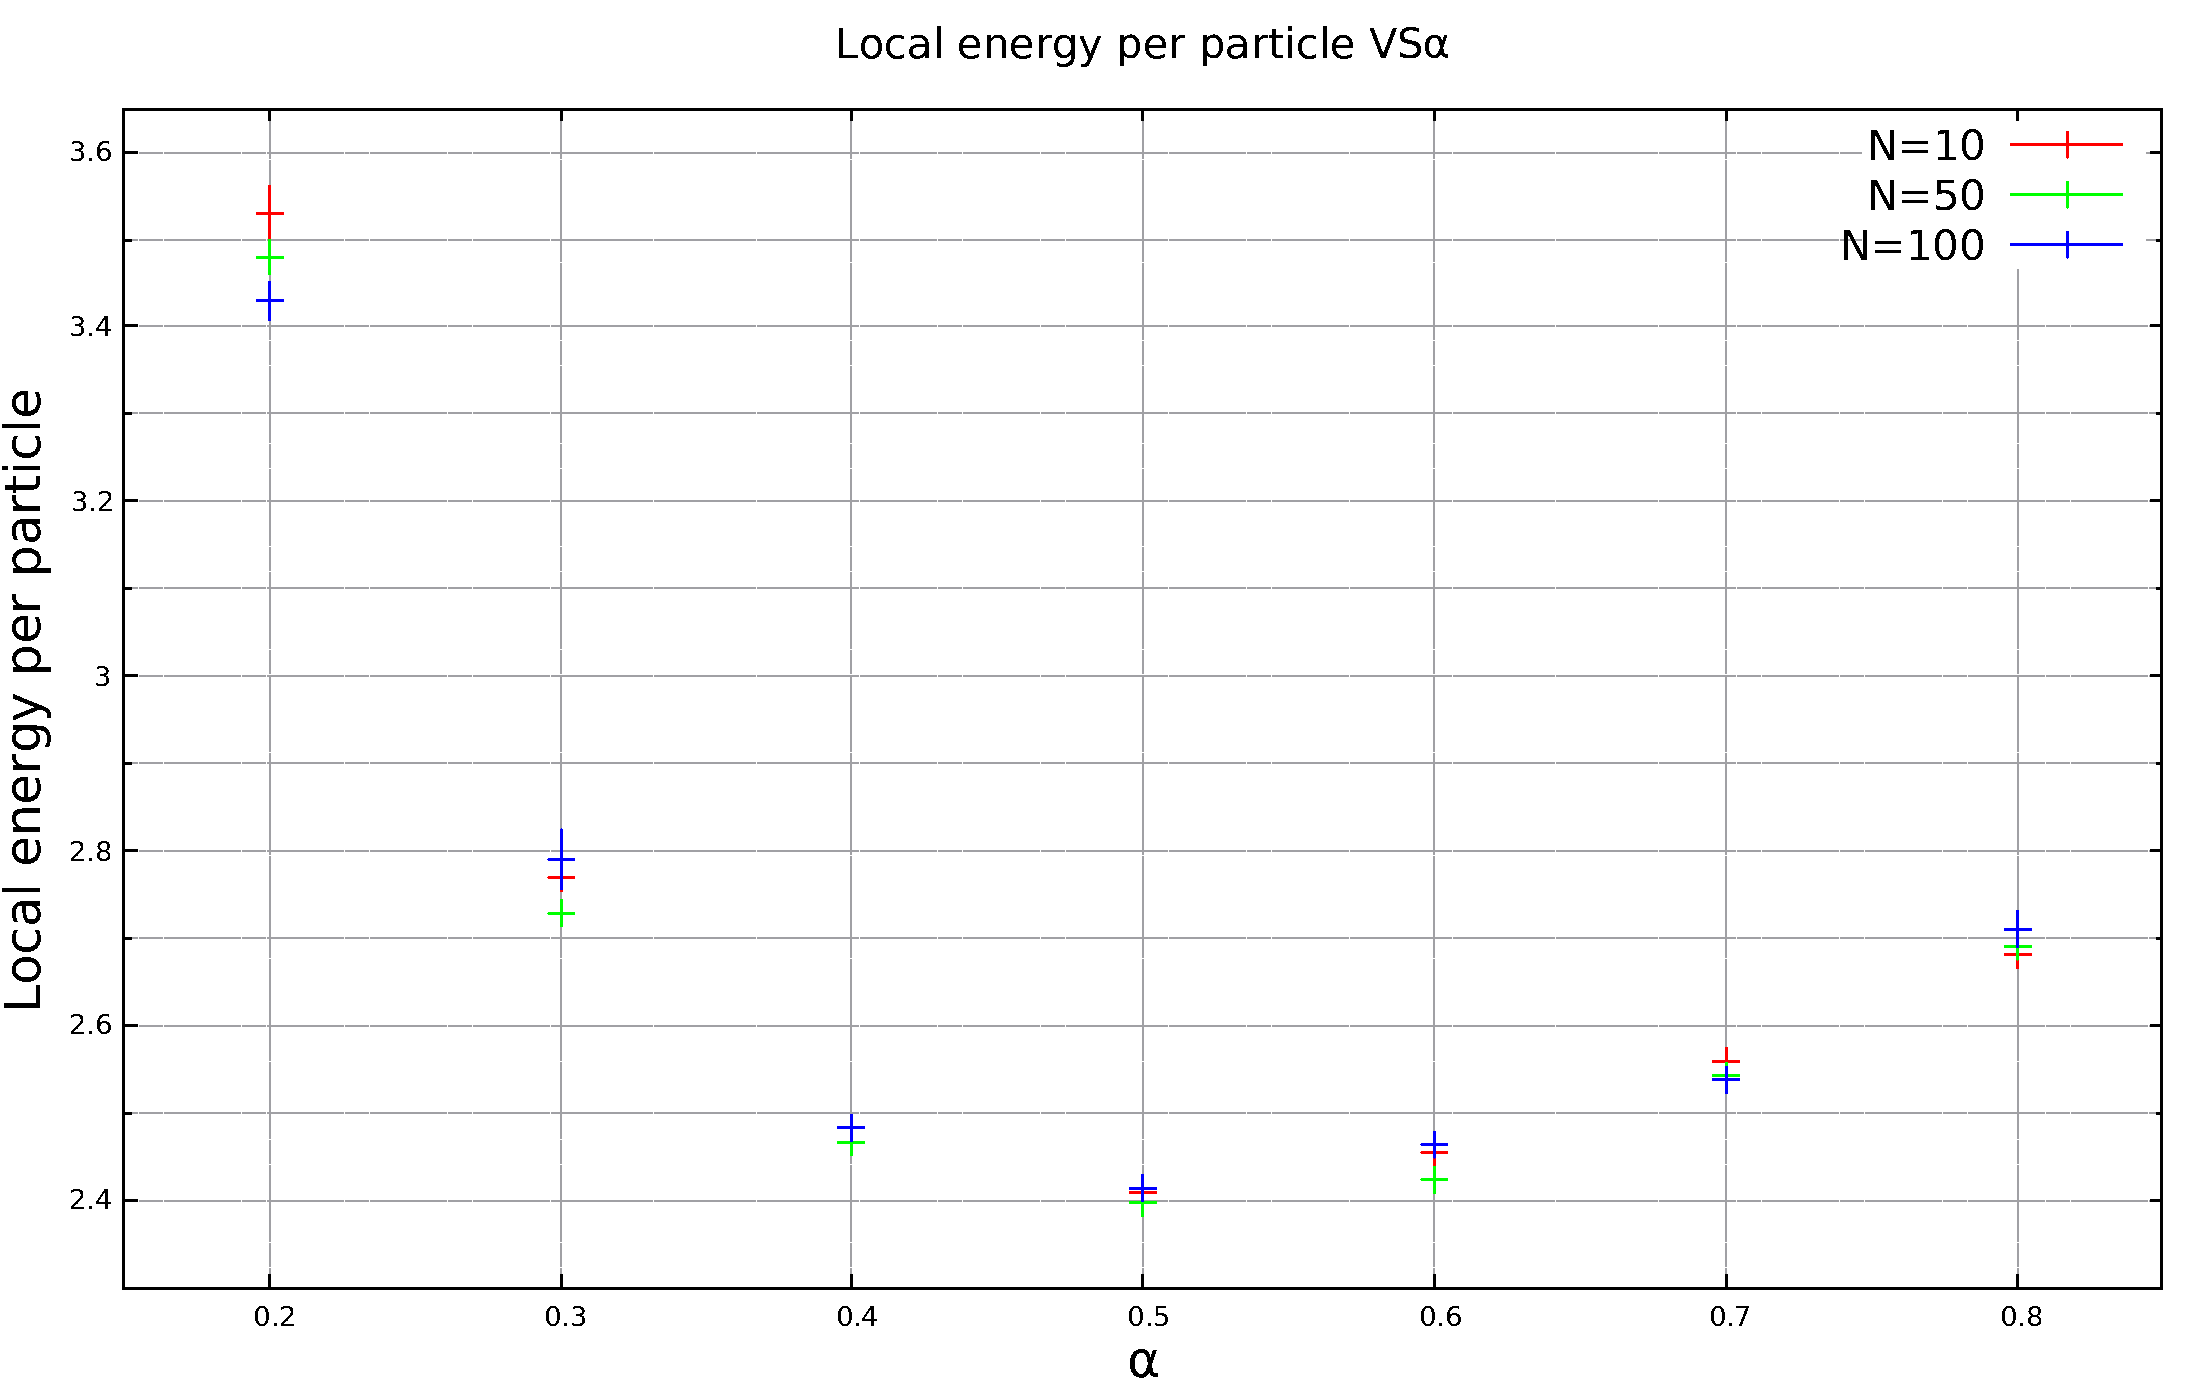
\includegraphics[scale = 0.5]{figures/en_alfa}}
\caption{Local energy per particle for different $\alpha$'s. The figure shows that the energy per particle for the most part is independent of the particle number. This breaks down at $\alpha = 0.2$.}
\label{fig_en_alfa}
\end{figure}

\subsection{Finding the optimal $\alpha$ using gradient descent}

The gradient descent method is applied to the interacting bosons to find the energy minimum. The results are presented in Fig. (\ref{fig_grad_minima}). Each data point is made using $10^5$ MC cycles. The initial guesses used for all the systems are $\alpha = 0.40$ and $\alpha = 0.60$. The location of the minimum can be found by taking the mean value of the $\alpha$ values after the method has converged. We are therefore interested in the region in Fig. (\ref{fig_grad_10_zoom}) where the blue and red dots overlap. By looking at the data this region can be set to $[0.50014, 0.500175]$. The mean $\alpha$ for the red dots is $\alpha = 0.50018 \pm (1.6\times 10^{-5})$ and for the blue dots is $\alpha = 0.50018 \pm (1.3\times10^{-5})$. By combining the data, the final answer becomes $\alpha_{optimal} = 0.50018 \pm (1\times10^{-5})$. 


\begin{figure}
	\centering
	\centerline{\resizebox{0.65\textwidth}{!}{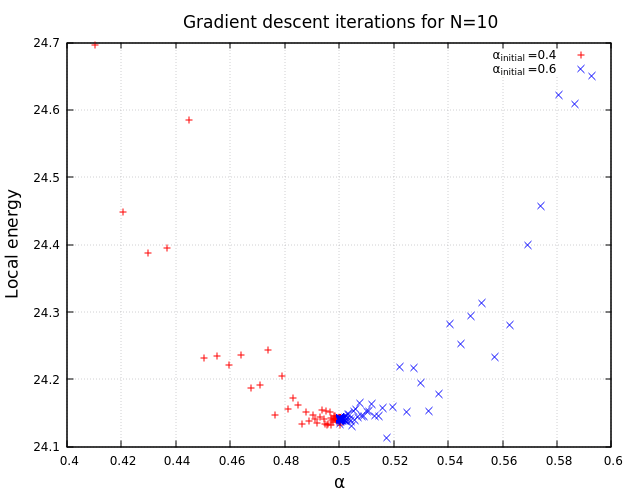
\includegraphics{figures/grad_desc_10_real_points}}
\resizebox{0.65\textwidth}{!}{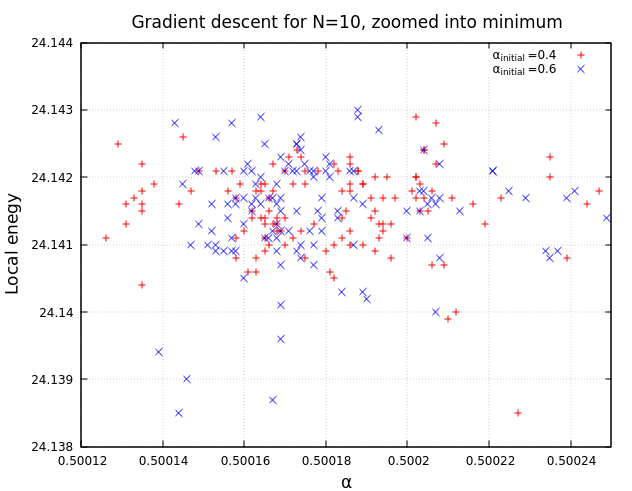
\includegraphics{figures/grad_desc_10_zoom_real_points}}}
	\centerline{\resizebox{0.65\textwidth}{!}{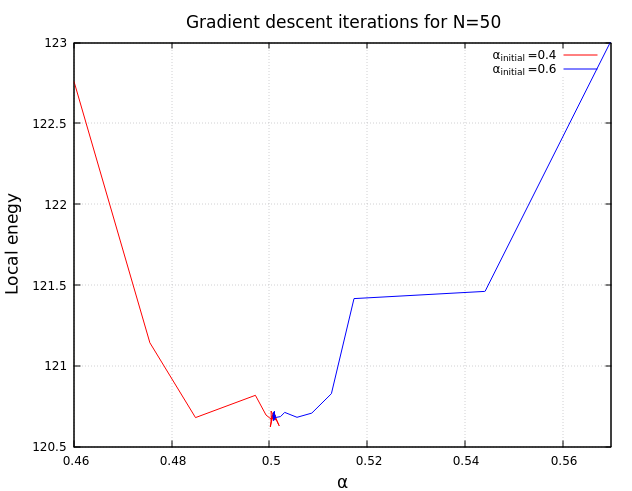
\includegraphics{figures/grad_desc_50_real}}
		\resizebox{0.65\textwidth}{!}{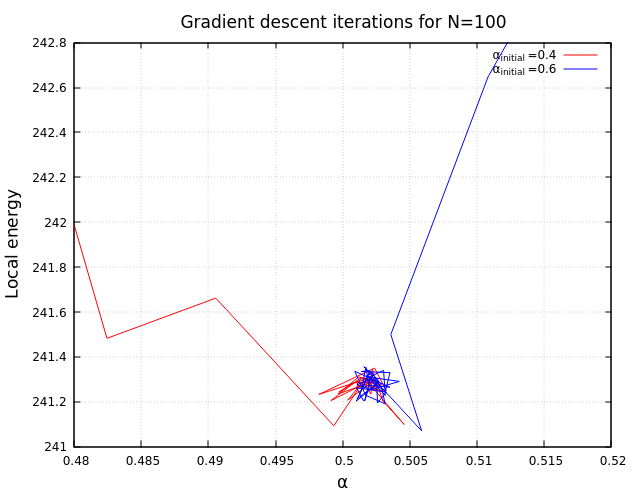
\includegraphics{figures/grad_desc_100_real}}}
%\begin{figure}[H]
%\centering
%\begin{subfigure}[t]{8cm}
%\centering
%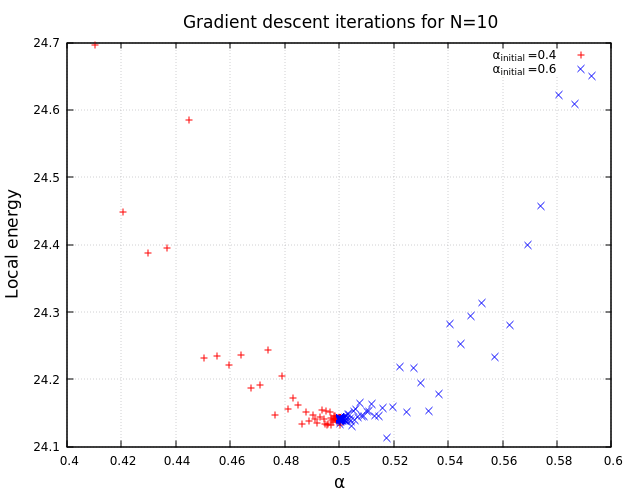
\includegraphics[width=8cm]{figures/grad_desc_10_real_points}
%        \caption{}\label{fig_grad_10}
%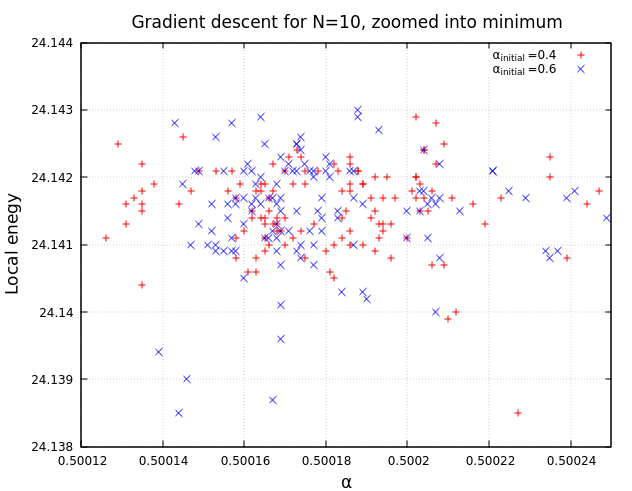
\includegraphics[width=8cm]{figures/grad_desc_10_zoom_real_points}
%\caption{}\label{fig_grad_10_zoom}
%\end{subfigure}
%\centering
%\begin{subfigure}[t]{8cm}
%\centering
%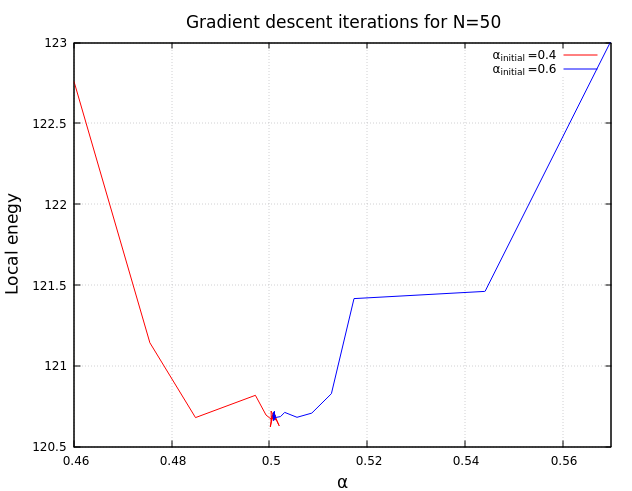
\includegraphics[width=8cm]{figures/grad_desc_50_real}
%        \caption{}\label{fig_grad_50}
%\end{subfigure}
%%
%\begin{subfigure}[t]{8cm}
%\centering
%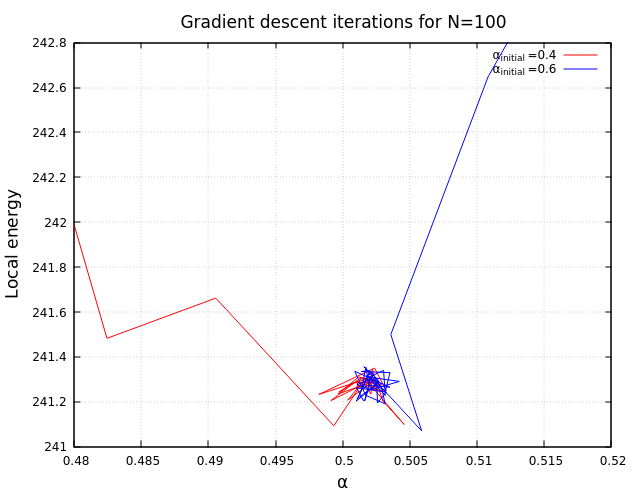
\includegraphics[width=8cm]{figures/grad_desc_100_real}
%\caption{}\label{fig_grad_100}
%\end{subfigure}
\caption{Gradient descent results from (a,b) 10, (c) 50, (d) 100 interacting bosons in an elliptical harmonic oscillator trap with $\beta = 2.82843$. The results were made using $\lambda = 0.001$. Fewer data points were used for the higher number of particles because of the large amount of time used to calculate the points.}
\label{fig_grad_minima}
\end{figure}

The same method can be applied to the $50$ and $100$ particle case. The data are presented in Fig. (\ref{fig_grad_50}) and Fig. (\ref{fig_grad_100}). 50 iterations are used in the 50 particle case and 30 iterations for the 100 particle case (for each initial $\alpha$). A good estimate for the optimal $\alpha$ is found by using the same procedure as in the 10 particle case. The results are presented in Tab. \ref{tab_optimal_alpha}, where we show also the ground state energies computed with these optimal variational parameters. The table shows that the optimal $\alpha$ tends to increase with the number of particles. This is a strange tendency. According to equation \ref{eq_psi}, one would expect the optimal $\alpha$ to be the same for all the $N$'s since the macroscopic wavefunction $\Psi(\textbf{r}, \alpha)$ is independent on $N$. The calculations for the spherical trap ($\beta = 1$) produce the same optimal $\alpha$'s. This fits with the theory.

The gradient descent method is also be applied to the system of non-interacting bosons. The algorithm finds $\alpha_{optimal} = 0.5 \pm (1\times10^{-6})$ in good agreement with the results in Fig. (\ref{fig_energy_minimum}) and the calculations in section \ref{section_non_interacting}.

%The ground state energies are also calculated with $10^5$ MC cycles. This should be fine as the calculations tend to give more precise energies, a tendency seen in table \ref{tab_energies_inter}.
\begin{table}[H]
\caption{Optimal variational parameters $\alpha$ for systems of interacting bosons found by using the gradient descent method together with the local energy computed using $10^6$ MC cycles. The data indicates that the optimal alpha increases with the number of particles.}
\centering
\begin{tabular}{ c c c}
\textbf{N}& \textbf{Optimal $\boldsymbol{\alpha}$}  & \textbf{Ground state local energy}\\ \hline
10 & $0.50018 \pm 0.00001$ &  $24.1917 \pm 0.0002$\\ 
50 & $0.50093\pm0.00001$     &  $120.929 \pm 0.005$ \\
100 & $0.5021 \pm 0.0006$    &   $241.77 \pm 0.02$  \\
\end{tabular}
\label{tab_optimal_alpha}
\end{table} 
